% !TEX program = xelatex
\documentclass[14pt,aspectratio=169]{beamer}
\usetheme{Singapore}
\usepackage[UTF8]{ctex}
\graphicspath{{Arquivos/}}
\usepackage[utf8]{inputenc}
% \usepackage[portuguese]{babel}
\usepackage[T1]{fontenc}
\usepackage{amsmath}
\usepackage{bookmark}
\usepackage{amsfonts}
\usepackage{amssymb}
\usepackage{graphicx}
\author{修格致}
\newcommand{\TT}{Spatial Interactions and Oscillatory TOCs}
\newcommand{\IN}{Introduction}
\newcommand{\PI}{I - Contribuir é Reconhececimento}
\newcommand{\PII}{II - Contribuir é Adoração}
\newcommand{\PIII}{III - Contribuir é Compromisso}
\newcommand{\PIV}{IV - Contribuir é Fidelidade}
\newcommand{\PV}{V - Contribuir é Confiança}
\newcommand{\CO}{Conclusion}

\title{\TT}
% \setbeamercovered{transparent} 
% \setbeamertemplate{navigation symbols}{\href{www.egmon.com.br}{www.egmon.com.br}} 
\logo{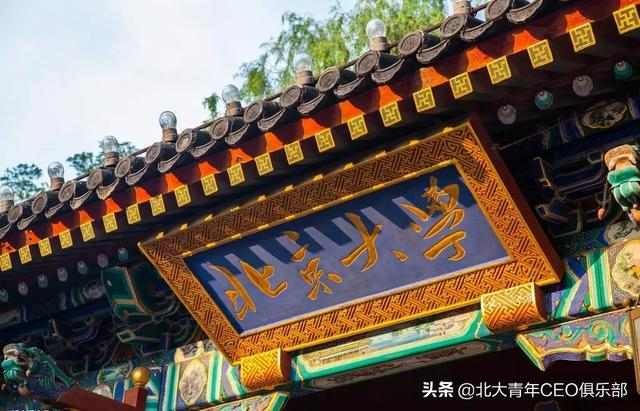
\includegraphics[scale=0.033]{LogoReformada}} 
\institute{IRSGIS\\Peking U} 
\date{\today}
\begin{document}

\begin{frame}
\titlepage
\end{frame}

\begin{frame}{Table of Contents}
    \tableofcontents
\end{frame}

\LARGE
\section{背景}
\begin{frame}{The Tragedy of the Commons}
\begin{quote}{Garratt Hardin:}
 \small
 \\
    The population problem has no technical solution;\\
it requires a fundamental extension in morality.
\end{quote}

\end{frame}

\begin{frame}{Q\&A for TOC}
\begin{itemize}
    \item What is?
    \begin{itemize}
        \item Two individuals choose amongst distinct strategies to utilize a limited public good.
    \end{itemize}
    \item Why is it a dilemma?
    \begin{itemize}
        \item Combined benefit: through cooperation.
        \item Personal benefit: through defection.
    \end{itemize}
\end{itemize}
\end{frame}

\begin{frame}{\TB}{\TT}
 \begin{block}{\DT}
4 O sacerdote tomará o cesto da tua mão e o porá diante do altar do SENHOR, teu Deus.
 \end{block}
\end{frame}

\begin{frame}{\TB}{\TT}
 \begin{block}{\DT}
 \Large
5 Então, testificarás perante o SENHOR, teu Deus, e dirás: Arameu prestes a perecer foi meu pai, e desceu para o Egito, e ali viveu como estrangeiro com pouca gente; e ali veio a ser nação grande, forte e numerosa.
 \end{block}
\end{frame}

\begin{frame}{\TB}{\TT}
 \begin{block}{\DT}
6 Mas os egípcios nos maltrataram, e afligiram, e nos impuseram dura servidão.
 \end{block}
\end{frame}

\begin{frame}{\TB}{\TT}
 \begin{block}{\DT}
7 Clamamos ao SENHOR, Deus de nossos pais; e o SENHOR ouviu a nossa voz e atentou para a nossa angústia, para o nosso trabalho e para a nossa opressão;
 \end{block}
\end{frame}

\begin{frame}{\TB}{\TT}
 \begin{block}{\DT}
8 e o SENHOR nos tirou do Egito com poderosa mão, e com braço estendido, e com grande espanto, e com sinais, e com milagres;
 \end{block}
\end{frame}

\begin{frame}{\TB}{\TT}
 \begin{block}{\DT}
9 e nos trouxe a este lugar e nos deu esta terra, terra que mana leite e mel.
 \end{block}
\end{frame}

\begin{frame}{\TB}{\TT}
 \begin{block}{\DT}
10 Eis que, agora, trago as primícias dos frutos da terra que tu, ó SENHOR, me deste. Então, as porás perante o SENHOR, teu Deus, e te prostrarás perante ele.
 \end{block}
\end{frame}

\begin{frame}{\TB}{\TT}
 \begin{block}{\DT}
11 Alegrar-te-ás por todo o bem que o SENHOR, teu Deus, te tem dado a ti e a tua casa, tu, e o levita, e o estrangeiro que está no meio de ti.
 \end{block}
\end{frame}

\begin{frame}{\TB}{\TT}
 \begin{block}{\DT}
 \Large
12 Quando acabares de separar todos os dízimos da tua messe no ano terceiro, que é o dos dízimos, então, os darás ao levita, ao estrangeiro, ao órfão e à viúva, para que comam dentro das tuas cidades e se fartem.
 \end{block}
\end{frame}

\begin{frame}{\TB}{\TT}
 \begin{block}{\DT}
 \Large
13 Dirás perante o SENHOR, teu Deus: Tirei de minha casa o que é consagrado e dei também ao levita, e ao estrangeiro, e ao órfão, e à viúva, segundo todos os teus mandamentos que me tens ordenado; nada transgredi dos teus mandamentos, nem deles me esqueci.
 \end{block}
\end{frame}

\begin{frame}{\TB}{\TT}
 \begin{block}{\DT}
 \Large
14 Dos dízimos não comi no meu luto e deles nada tirei estando imundo, nem deles dei para a casa de algum morto; obedeci à voz do SENHOR, meu Deus; segundo tudo o que me ordenaste, tenho feito.
 \end{block}
\end{frame}

\begin{frame}{\TB}{\TT}
 \begin{block}{\DT}
15 Olha desde a tua santa habitação, desde o céu, e abençoa o teu povo, a Israel, e a terra que nos deste, como juraste a nossos pais, terra que mana leite e mel. 
 \end{block}
\end{frame}

\begin{frame}
 \tableofcontents
\end{frame}

\section{\IN}
\begin{frame}{\IN}{\TT}
 \begin{table}
  \begin{center}
   \begin{tabular}{lr}
   \multicolumn{2}{c}{\textbf{DOIS EXTREMOS}}\\ \pause
   O Legalista \pause & O Negligente    
   \end{tabular}
  \end{center}
 \end{table}
\end{frame}

\begin{frame}{\IN}{\TT}
 A Bíblia apresenta as seguintes formas de contribuições:
\end{frame}

\begin{frame}{\IN}{\TT}
 \begin{itemize}
  \item \textbf{Primícias} \pause - Apresentação, ao Senhor, dos primeiros frutos da colheita.
  \item[] Dt 26.2
 \end{itemize}
\end{frame}

\begin{frame}{\IN}{\TT}
 \begin{itemize}
  \item \textbf{Dízimos} \pause - Contribuição referente à décima parte da produção dos frutos da terra, dos rebalhos e das rendas em geral.
  \item[] Gn 28.20-22; Lv 27.30-34
 \end{itemize}
\end{frame}

\begin{frame}{\IN}{\TT}
 \begin{itemize}
  \item \textbf{Ofertas} \pause - Contribuições voluntárias e esporádicas, de qualquer espécie, para fins específicos.
  \item[] Ed 2.68-69
 \end{itemize}
\end{frame}

\begin{frame}{\IN}{\TT}
 \begin{itemize}
  \item \textbf{Esmolas} \pause - Doações destinadas ao alívio imediato de carências de pessoas necessitadas.
  \item[] At 10.1-2
 \end{itemize}
\end{frame}

\section{\PI}
\begin{frame}{\PI}{\TT}\pause
 \textbf{Primícias} - A apresentação dessas ofertas ao Senhor é uma expressão de reconhecimento de que, Deus está por trás de todo o salário que vem do nosso trabalho.
\end{frame}

\begin{frame}{\PI}{\TT}
 Toda sorte de bênçãos procede do Senhor:\pause
 \begin{block}{Tiago 1.17a}
 Toda boa dádiva e todo dom perfeito são lá do alto, do Pai das Luzes.
 \end{block}
\end{frame}

\begin{frame}{\PI}{\TT}
 Quando contribuímos, devemos fazê-lo como demonstração de um profundo reconhecimento de que tudo o que recebemos e possuímos foi concedido por Deus.
\end{frame}

\begin{frame}{\PI}{\TT}
 \begin{block}{I Crônicas 29.14}
 Porque quem sou eu, e quem é o meu povo para que pudéssemos dar voluntariamente estas coisas? Porque tudo vem de ti, e das tuas mãos to damos.
 \end{block}
\end{frame}

\begin{frame}{\PI}{\TT}
 \begin{block}{I Crônicas 21.23-24}\pause
 \Large
23 Então, disse Ornã a Davi: Tome-a o rei, meu senhor, para si e faça dela o que bem lhe parecer; eis que dou os bois para o holocausto, e os trilhos, para a lenha, e o trigo, para oferta de manjares; dou tudo.
 \end{block}
\end{frame}

\begin{frame}{\PI}{\TT}
 \begin{block}{I Crônicas 21.23-24}
24 Tornou o rei Davi a Ornã: Não; antes, pelo seu inteiro valor a quero comprar; porque não tomarei o que é teu para o SENHOR, nem oferecerei holocausto que não me custe nada.
 \end{block}
\end{frame}

\section{\PII}
 \begin{frame}{\PII}{\TT}\pause
 A contribuição para a obra de Deus não pode ser confundida com um \textbf{imposto} ou uma \textbf{taxa} ao qual somos obrigados a pagar.
 \end{frame}

\begin{frame}{\PII}{\TT}
 \begin{block}{Deuteronômio 14.22-23}
 22 Certamente, darás os dízimos de todo o fruto das tuas sementes, que ano após ano se recolher do campo.
 \end{block}
\end{frame}

\begin{frame}{\PII}{\TT}
 \begin{block}{Deuteronômio 14.22-23}
\Large 
23 E, perante o SENHOR, teu Deus, no lugar que escolher para ali fazer habitar o seu nome, comerás os dízimos do teu cereal, do teu vinho, do teu azeite e os primogênitos das tuas vacas e das tuas ovelhas; para que aprendas a temer o SENHOR, teu Deus, todos os dias.
 \end{block}
\end{frame}

\begin{frame}{\PII}{\TT}
 \begin{itemize}
  \item Se Deus não precisa do meu dinheiro;\pause
  \item Se Ele é capaz de criar todas as coisas;\pause
  \item Então, por que Ele quer que eu entregue o meu Dízimo?
 \end{itemize}
\end{frame}

\begin{frame}{\PII}{\TT}
 \begin{block}{Deuteronômio 14.23b}
Para que aprendas a temer o SENHOR, teu Deus, todos os dias.
 \end{block}
\end{frame}

\begin{frame}{\PII}{\TT}
 \begin{block}{II Coríntios 9.7}
Cada um contribua segundo tiver proposto no coração, não com tristeza ou por necessidade; porque Deus ama a quem dá com alegria.
  \end{block}
\end{frame}

\begin{frame}{\PII}{\TT}
 \begin{itemize}
  \item A contibuição deve ser:\pause
   \begin{enumerate}
   \Large
    \item Voluntária;\pause
    \item Com alegria;\pause
    \item Com devoção a Deus.
   \end{enumerate}    
 \end{itemize}
 \begin{center}
Porque Deus ama a quem dá com alegria.
 \end{center}
\end{frame}

\section{\PIII}
\begin{frame}{\PIII}{\TT}\pause
 \begin{itemize}
  \item Os recursos que \textbf{Deus nos dá}, não podem ser retidos de forma egoísta;\pause
  \item Devem ser uma aplicação social;\pause
  \item Devem ser partilhados.
 \end{itemize}
\end{frame}

\begin{frame}{\PIII}{\TT}
 \begin{itemize}
  \item Os dízimos devem atender a 3 necessidades básicas:
 \end{itemize}
\end{frame}

\begin{frame}{\PIII}{\TT}
 \begin{enumerate}
  \item[1 -] Manutenção do culto;\pause
 \end{enumerate}
 \begin{block}{Números 18.21}
 Aos filhos de Levi dei todos os dízimos em Israel por herança, pelo serviço que prestam, serviço da tenda da congregação.
 \end{block}
\end{frame}

\begin{frame}{\PIII}{\TT}
 \begin{block}{Malaquias 3.10}
\Large
Trazei todos os dízimos à casa do Tesouro, para que haja mantimento na minha casa; e provai-me nisto, diz o SENHOR dos Exércitos, se eu não vos abrir as janelas do céu e não derramar sobre vós bênção sem medida.
 \end{block}
\end{frame}

\begin{frame}{\PIII}{\TT}
 \textbf{Malaquias 3.10 nos ensina:}\pause
 \begin{enumerate}
  \item[1º] Os Dízimos são entregues exclusivamente no Templo:\pause
 \end{enumerate}
  \begin{center}
  \textcolor{red}{Trazei todos os dízimos à casa do Tesouro}
  \end{center} 
\end{frame}

\begin{frame}{\PIII}{\TT}
 \textbf{Malaquias 3.10 nos ensina:}
 \begin{enumerate}
  \item[2º] Como os Dízimos devem ser administrados:\pause
 \end{enumerate}
  \begin{center}
  \textcolor{red}{Para que haja mantimento na minha casa}
  \end{center}
\end{frame}

\begin{frame}{\PIII}{\TT}
 \textbf{Malaquias 3.10 nos ensina:}
 \begin{enumerate}
  \item[3º] Há consequências para os fiéis:\pause  
 \end{enumerate}
  \begin{center}
  \textcolor{red}{Provai-me nisto, diz o SENHOR dos Exércitos, se eu não vos abrir as janelas do céu e não derramar sobre vós bênção sem medida.}
  \end{center}
\end{frame}

\begin{frame}{\PIII}{\TT}
 \begin{itemize}
     \item A Bíblia não diz que você será amaldiçoado ou que irá para o inferno caso deixe de dizimar;\pause
     \item Mas ela é clara ao dizer que há privações de bênçãos aos infiéis em dizimar!
 \end{itemize}
\end{frame}

\begin{frame}{\PIII}{\TT}
 \begin{enumerate}
  \item[2 -] Assistência aos necessitados;
 \end{enumerate}
\end{frame}

\begin{frame}{\PIII}{\TT}
 \begin{block}{Atos 4.32-35}
32 Da multidão dos que creram era um o coração e a alma. Ninguém considerava exclusivamente sua nem uma das coisas que possuía; tudo, porém, lhes era comum.
 \end{block}
\end{frame}

\begin{frame}{\PIII}{\TT}
 \begin{block}{Atos 4.32-35}
33 Com grande poder, os apóstolos davam testemunho da ressurreição do Senhor Jesus, e em todos eles havia abundante graça.
 \end{block}
\end{frame}

\begin{frame}{\PIII}{\TT}
 \begin{block}{Atos 4.32-35}
34 Pois nenhum necessitado havia entre eles, porquanto os que possuíam terras ou casas, vendendo-as, traziam os valores correspondentes
 \end{block}
\end{frame}

\begin{frame}{\PIII}{\TT}
 \begin{block}{Atos 4.32-35}
35 e depositavam aos pés dos apóstolos; então, se distribuía a qualquer um à medida que alguém tinha necessidade.
 \end{block}
\end{frame}

\begin{frame}{\PIII}{\TT}
 \begin{enumerate}
  \item[3 -] Fortalecimento da Vida comunitária;\pause
  \begin{itemize}
   \Large
   \item Haviam grandes festas de confraternização entre eles.
  \end{itemize}
 \end{enumerate}
\end{frame}

\begin{frame}{\PIII}{\TT}
 \begin{block}{Deuteronômio 26.11}
Alegrar-te-ás por todo o bem que o SENHOR, teu Deus, te tem dado a ti e a tua casa, tu, e o levita, e o estrangeiro que está no meio de ti.
 \end{block}
\end{frame}

\section{\PIV}
\begin{frame}{\PIV}{\TT}

\end{frame}

\section{\PV}
\begin{frame}{\PV}{\TT}

\end{frame}

\section{\CO}
\begin{frame}{\CO}{\TT}

\end{frame}


\logo{}
\small
\begin{frame}
 \begin{minipage}{0.45\linewidth}
  \begin{figure}
   \begin{center}
    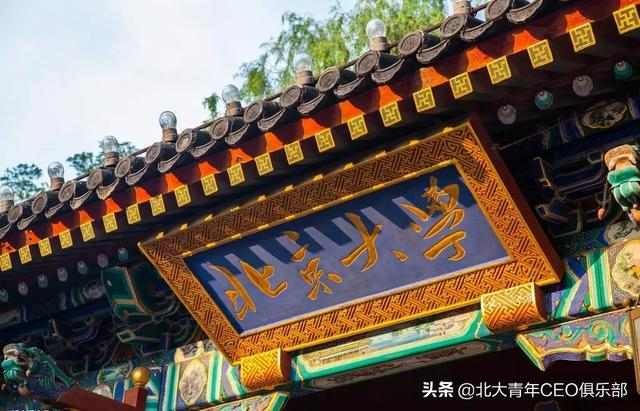
\includegraphics[scale=0.2]{LogoReformada}
   \end{center}
  \end{figure}
 \end{minipage}
 \begin{minipage}{0.45\linewidth}
  \begin{figure}
   \begin{center}
    
\includegraphics[scale=0.5]{Sarca}
   \end{center}
  \end{figure}
 \end{minipage}
\begin{center}
Download do Slide em: \href{www.egmon.com.br}{www.egmon.com.br}
\end{center}
\end{frame}


\end{document}